\documentclass[journal]{IEEEtran}

% Additional packages
\usepackage{graphicx}
\usepackage{amsmath}
\usepackage{hyperref}
\usepackage{float}
\usepackage{subcaption}
\usepackage{booktabs}
\usepackage{pgfplotstable}
\usepackage{qrcode}

\pgfplotsset{compat=1.18}

\begin{document}

\title{Investigation of the Magnetic Field of a Solenoid}
\author{IBRAHIM H.I. ABUSHAWISH \\
Istanbul University, Department of Physics \\
Instructor: Res. Asst. Dilan AKHAN \\
Experiment Date: 4.11.2024, Report Submission Date: 02.12.2024\\
Course \& Section Number: PHYS2305}

\maketitle

\begin{abstract}
This report investigates the magnetic field of a solenoid, focusing on experimentally determining the permeability of free space (\( \mu_0 \)) by comparing theoretical models with measured data. The experiment examines the magnetic flux density (\( B \)) both inside and outside a solenoid as a function of current (\( I \)), coil geometry (turns per unit length \( n \)), and distance (\( x \)). By analyzing raw data, plotting relationships, and calculating \( \mu_0 \), the results validate theoretical predictions, demonstrating consistency between experimental findings and established electromagnetic theory.
\end{abstract}

\section{Introduction}
The magnetic field generated by a solenoid is a fundamental concept in electromagnetism, with applications in inductors, electromagnets, and transformers. The strength and behavior of this field depend on factors such as the current (\( I \)) flowing through the solenoid, the number of turns per unit length (\( n \)), and the geometry of the coil. The relationship for the magnetic field inside an ideal solenoid is given by:
\begin{equation}
    B = \mu_0 n I, \label{eq:ideal_field}
\end{equation}
where \( B \) is the magnetic flux density, \( \mu_0 \) is the permeability of free space (\( 4\pi \times 10^{-7} \, \mathrm{N \cdot A^{-2}} \)), \( n \) is the number of turns per unit length, and \( I \) is the current through the solenoid.

For points outside the solenoid or along its axis, the Biot-Savart law provides a generalized expression for the magnetic field:
\begin{equation}
    d\mathbf{B} = \frac{\mu_0}{4\pi} \frac{I d\mathbf{l} \times \mathbf{r}}{|\mathbf{r}|^3}, \label{eq:biot_savart}
\end{equation}
where \( d\mathbf{l} \) is an infinitesimal current element, and \( \mathbf{r} \) is the distance vector from the current element to the point of observation.

The aim of this experiment is to measure the magnetic flux density inside and outside a solenoid and determine \( \mu_0 \) by analyzing the relationship between \( B \), \( n \), and \( I \). Equation~\eqref{eq:ideal_field} is used to model the field inside the solenoid, while Equation~\eqref{eq:biot_savart} serves as a theoretical basis for analyzing the field outside the solenoid.

\section{Experimental Procedure}
The experiment was conducted in two parts to investigate the magnetic field inside and outside a solenoid. The experimental setups for these parts are depicted in Figures~\ref{fig:Outside_setup} and~\ref{fig:Inside_setup}.

\subsection{Part One: Magnetic Field Outside the Solenoid}
The first part of the experiment focused on measuring the magnetic field outside the solenoid. The setup, shown in Figure~\ref{fig:Outside_setup}, consisted of a solenoid, a variable direct current source, an ammeter, and a compass needle. The compass needle was aligned along the north-south direction, pointing to zero degrees, while the solenoid was positioned in the west-east direction, with its axis aligned toward the compass needle.

To begin, a maximum current of approximately \( 1.5 \, \text{A} \) was passed through the solenoid, and the distance between the solenoid and the compass needle was adjusted until the needle deviated by about \( 70^\circ \). The current was then reset to zero. Various current values were applied through the solenoid, and for each current, the deviation angle (\( \alpha \)) of the compass needle was measured and recorded.

Using the horizontal component of the Earth's magnetic field (\( B_H = 26 \, \mu T \)), the magnetic field intensity (\( B \)) created by the solenoid for each current was calculated using:
\begin{equation}
    B = B_H \tan \alpha, \label{eq:field_outside}
\end{equation}
where \( \tan \alpha \) is derived from the measured deviation angle. The calculated values were tabulated, and the relationship between current and deviation angle (\( I = f(\alpha) \)) was plotted for analysis, as shown in Figure~\ref{fig:current_vs_tan_alpha}.

\begin{figure}[H]
    \centering
    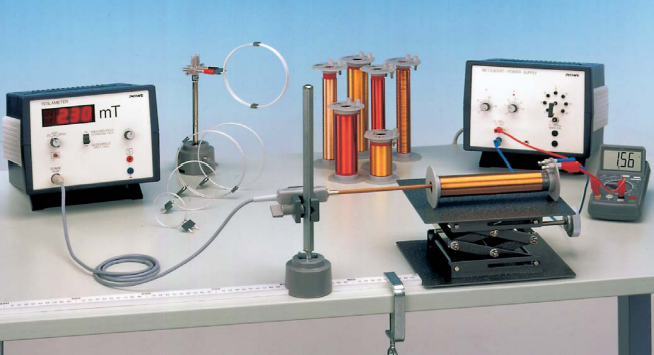
\includegraphics[width=\linewidth]{IMAGES/Biot-Savart_experimen_setup.png}
    \caption{Experimental setup for measuring the magnetic field outside the solenoid. The compass needle is used to measure deviation angles for various currents.}
    \label{fig:Outside_setup}
\end{figure}

\subsection{Part Two: Magnetic Field Inside the Solenoid}
The second part of the experiment measured the magnetic field inside the solenoid. The experimental setup, shown in Figure~\ref{fig:Inside_setup}, included a solenoid, a variable power supply, a Tesla meter, and a ruler. A constant current of \( 0.5 \, \text{A} \) was applied through the solenoid to ensure consistent measurement conditions.

The magnetic flux density (\( B \)) was measured at various distances along the solenoid's axis by moving the Tesla meter along the \( x \)-axis. These measurements were taken for a fixed current of \( I = 1 \, \text{A} \), and the resulting data was used to plot \( B(x) \), showing the relationship between magnetic flux density and distance from the solenoid's center.

To analyze the influence of coil properties, \( B(x) \) curves were generated for coils with different numbers of turns (\( n = 75, 150, 300 \)) but fixed diameter (\( 2a = 26 \, \text{mm} \)) and length (\( l = 160 \, \text{mm} \)). Additionally, \( B(x) \) graphs were plotted for coils with the same number of turns (\( n = 300 \)) but varying diameters (\( 2a = 26, 33, 41 \, \text{mm} \)).

Finally, the permeability of free space (\( \mu_0 \)) was determined by plotting \( B(n) \), the magnetic flux density as a function of the number of turns for a fixed distance \( x \). The slope of the resulting line provided the experimental value of \( \mu_0 \), validating Equation~\eqref{eq:ideal_field}.

\begin{figure}[H]
    \centering
    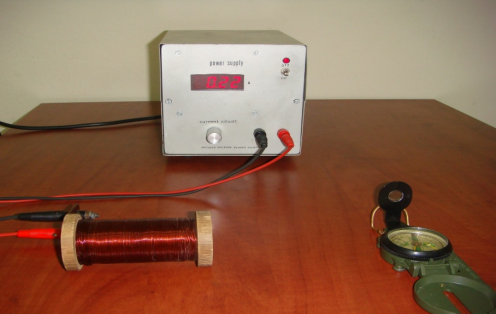
\includegraphics[width=\linewidth]{IMAGES/Multi-turn_Coi_Experimental_setup.png}
    \caption{Experimental setup for measuring the magnetic field inside the solenoid. A Tesla meter is used to measure magnetic flux density along the solenoid axis.}
    \label{fig:Inside_setup}
\end{figure}

    
    \section{Results}

    The results of this experiment are presented in two parts, corresponding to the magnetic field measurements outside and inside the solenoid. The analysis includes raw data, derived calculations, and regression models to validate theoretical predictions and determine key parameters, including the permeability of free space (\( \mu_0 \)).
    
    \subsection{Part One: Magnetic Field Outside the Solenoid}
    Table~\ref{tab:outside_data} summarizes the measured deviation angles (\( \alpha \)) and the corresponding calculated magnetic field values (\( B \)) for various currents (\( I \)). Using the relationship \( B = B_H \tan \alpha \) (Equation~\ref{eq:field_outside}), the magnetic flux density was computed based on the horizontal component of Earth's magnetic field (\( B_H = 26 \, \mu T \)).


    \begin{table}[H]
        \centering
        \caption{Magnetic Field Outside the Solenoid}
        \label{tab:outside_field}
        \begin{tabular}{cccc}
        \hline
        Current ($I$, A) & Deviation Angle ($\alpha$, °) & $\tan(\alpha)$ & Magnetic Field ($B$, $\mu T$) \\ \hline
        0.0 & 0  & 0.000 & 0.000 \\
        0.2 & 14 & 0.249 & 6.483 \\
        0.4 & 26 & 0.488 & 12.681 \\
        0.6 & 36 & 0.727 & 18.890 \\
        0.8 & 48 & 1.111 & 28.876 \\
        1.0 & 56 & 1.483 & 38.547 \\
        1.2 & 62 & 1.881 & 48.899 \\
        1.4 & 68 & 2.475 & 64.352 \\
        1.6 & 72 & 3.078 & 80.020 \\
        1.8 & 73 & 3.271 & 85.042 \\
        2.0 & 78 & 4.705 & 122.320 \\ \hline
        \end{tabular}
        \end{table}
        
        
        
    
    The relationship between current (\( I \)) and the tangent of the deviation angle (\( \tan \alpha \)) was analyzed using linear regression. The resulting model is shown in Figure~\ref{fig:current_vs_tan_alpha}, confirming a strong linear correlation.
    
    \begin{figure}[H]
    \centering
    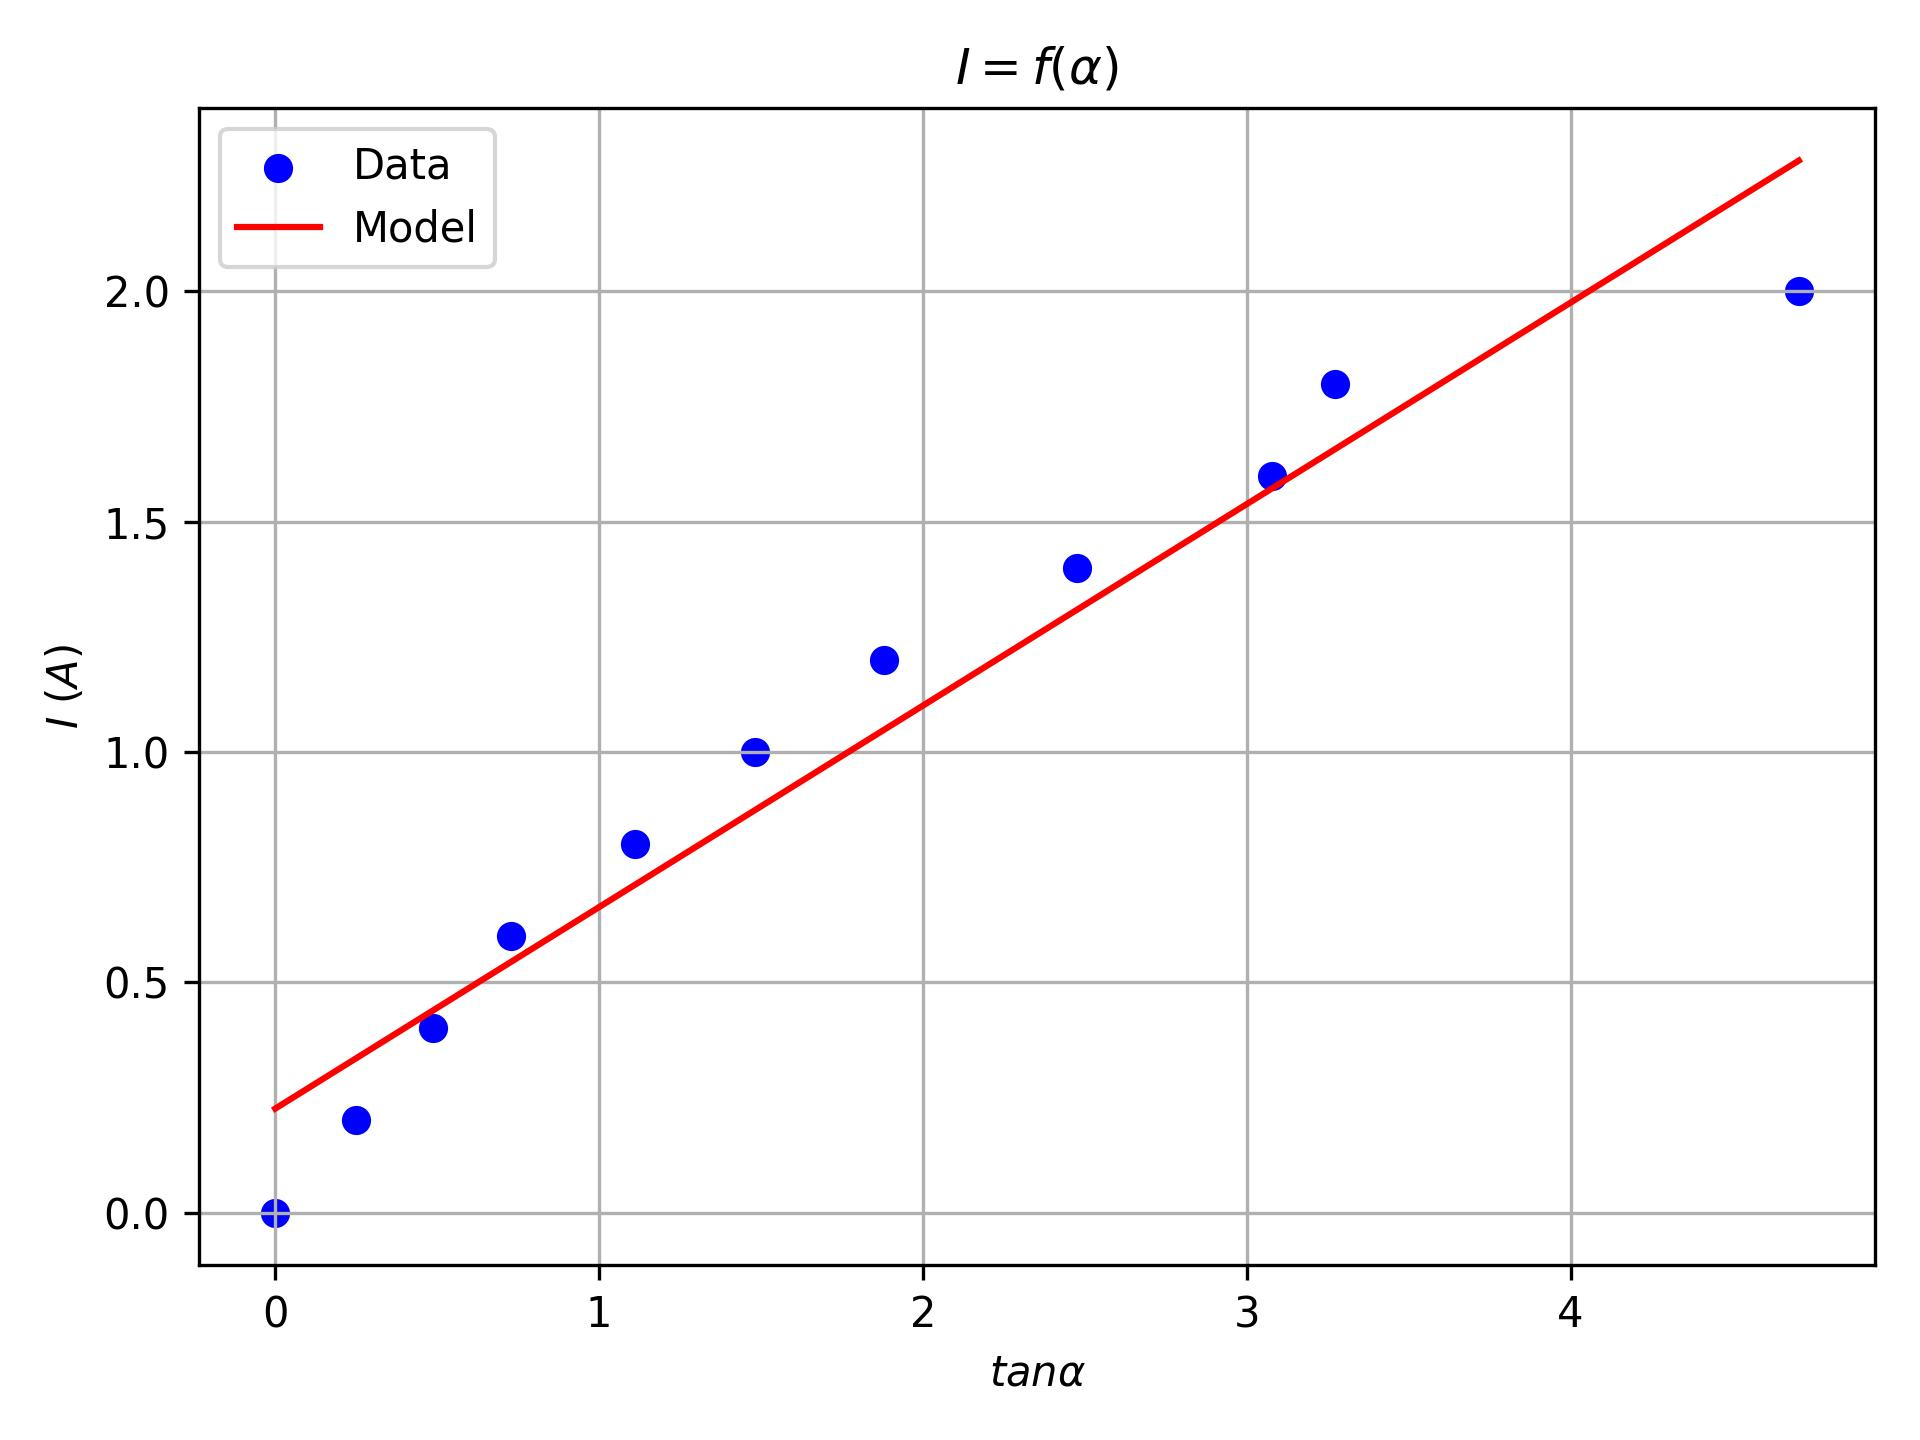
\includegraphics[width=\linewidth]{output_plots/current_vs_tan_alpha.jpg}
    \caption{Relationship between current (\( I \)) and tangent of deviation angle (\( \tan \alpha \)) outside the solenoid.}
    \label{fig:current_vs_tan_alpha}
    \end{figure}
    
    \subsection{Part Two: Magnetic Field Inside the Solenoid}
    For the second part, the magnetic flux density (\( B \)) inside the solenoid was measured at various distances (\( x \)) along its axis. Table~\ref{tab:inside_data} shows the raw data for one configuration (\( n = 150 \), \( 2a = 26 \, \text{mm} \)), while Figure~\ref{fig:fields_vs_distance} visualizes the field distributions for multiple configurations.
    
    \begin{table*}[t]
        \centering
        \caption{Magnetic Field Inside the Solenoid for Various Configurations}
        \label{tab:inside_field}
        \resizebox{\linewidth}{!}{
        \begin{tabular}{cccccc}
        \hline
        Distance ($x$, mm) & $n = 75, 2a = 26$ mm & $n = 150, 2a = 26$ mm & $n = 300, 2a = 26$ mm & $n = 300, 2a = 33$ mm & $n = 300, 2a = 41$ mm \\ \hline
        0   & 0.02 & 0.00 & 0.00 & 0.00 & 0.00 \\
        10  & 0.02 & 0.02 & 0.02 & 0.02 & 0.10 \\
        20  & 0.03 & 0.03 & 0.07 & 0.08 & 0.22 \\
        30  & 0.04 & 0.12 & 0.27 & 0.23 & 0.48 \\
        40  & 0.11 & 0.34 & 0.68 & 0.53 & 0.72 \\
        50  & 0.21 & 0.47 & 0.97 & 0.84 & 0.91 \\
        60  & 0.25 & 0.53 & 1.07 & 0.98 & 1.00 \\
        70  & 0.28 & 0.54 & 1.09 & 1.06 & 1.02 \\
        80  & 0.28 & 0.55 & 1.12 & 1.09 & 1.06 \\
        90  & 0.28 & 0.55 & 1.12 & 1.09 & 1.06 \\
        100 & 0.28 & 0.55 & 1.12 & 1.09 & 1.05 \\
        110 & 0.28 & 0.55 & 1.12 & 1.10 & 1.05 \\
        120 & 0.28 & 0.55 & 1.12 & 1.10 & 1.06 \\
        130 & 0.28 & 0.55 & 1.12 & 1.10 & 1.07 \\
        140 & 0.28 & 0.55 & 1.12 & 1.10 & 1.06 \\
        150 & 0.27 & 0.55 & 1.11 & 1.10 & 1.06 \\
        160 & 0.25 & 0.54 & 1.09 & 1.08 & 1.03 \\
        170 & 0.24 & 0.53 & 1.08 & 1.05 & 1.00 \\
        180 & 0.23 & 0.48 & 1.02 & 1.00 & 0.90 \\
        190 & 0.20 & 0.37 & 0.88 & 0.90 & 0.77 \\
        200 & 0.12 & 0.14 & 0.46 & 0.60 & 0.45 \\
        210 & 0.02 & 0.02 & 0.15 & 0.28 & 0.21 \\
        220 & 0.00 & 0.00 & 0.00 & 0.04 & 0.12 \\ \hline
        \end{tabular}
        }
        \end{table*}
        
        
    
    \begin{figure}[H]
    \centering
    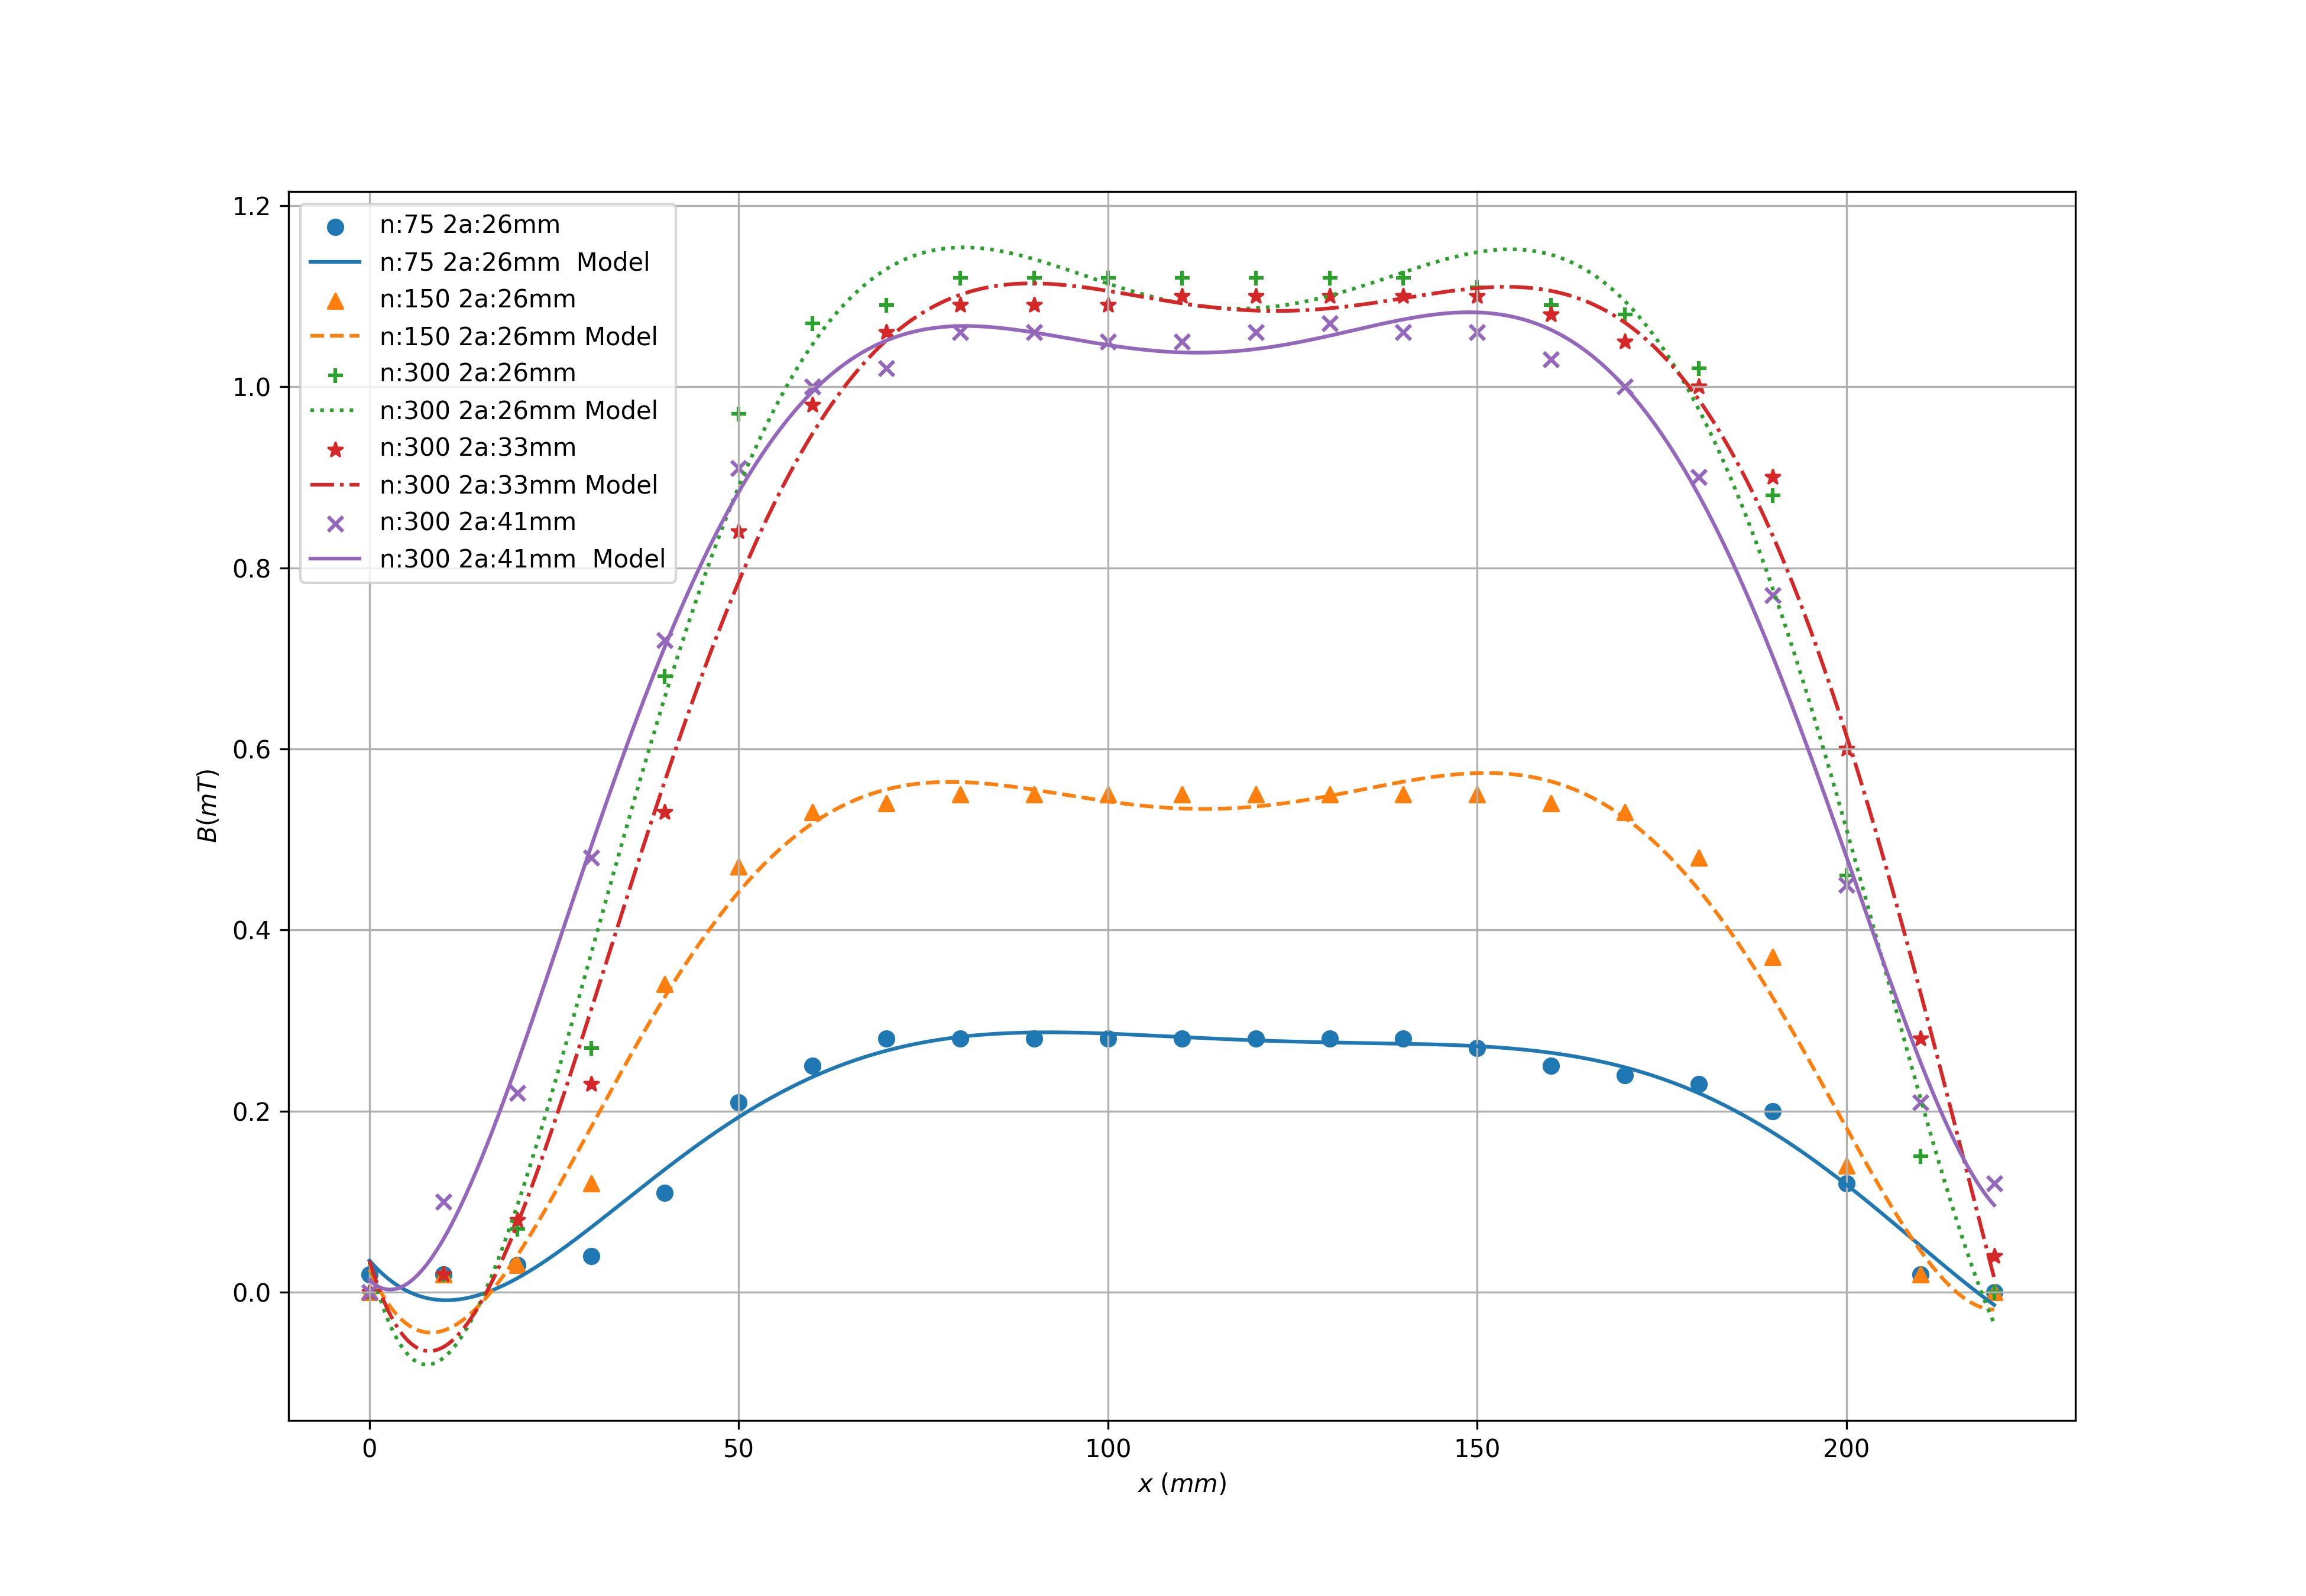
\includegraphics[width=\linewidth]{output_plots/Magnatic_Feilds_vs_distance.jpg}
    \caption{Magnetic field (\( B \)) as a function of distance (\( x \)) for various solenoid configurations.}
    \label{fig:fields_vs_distance}
    \end{figure}
    
    \subsection{Determination of \( \mu_0 \)}

    The permeability of free space (\( \mu_0 \)) was determined by analyzing the relationship between the magnetic flux density (\( B \)) and the number of turns (\( N \)) for a fixed distance (\( x = 110 \, \text{mm} \)). The linear regression model shown in Figure~\ref{fig:b_vs_turns} provides the slope, which can be used to calculate \( \mu_0 \) directly. The relationship is governed by the equation:
    
    \begin{equation}
        B = \mu_0 n I \implies \mu_0 = \frac{B}{n I},
    \end{equation}
    
    where \( n = \frac{N}{l} \) is the number of turns per unit length, \( I = 0.5 \, \text{A} \) is the applied current, and \( l = 160 \, \text{mm} = 0.16 \, \text{m} \) is the length of the solenoid. 
    
    Using the slope of the regression line in Figure~\ref{fig:b_vs_turns}, \( \text{slope} = 3.54 \times 10^{-6} \, \text{T/turn} \), we can calculate \( \mu_0 \) as follows:
    
    \begin{equation}
        \mu_0 = \frac{\text{slope} \cdot l}{I}.
    \end{equation}
    
    Substituting the values:
    \begin{align*}
        \mu_0 &= \frac{(3.54 \times 10^{-6} \, \text{T/turn}) \cdot (0.16 \, \text{m})}{0.5 \, \text{A}} \\
        \mu_0 &= 1.13 \times 10^{-6} \, \text{H/m}.
    \end{align*}
    
    This experimentally determined value of \( \mu_0 \) closely aligns with the theoretical value of \( \mu_0 = 4\pi \times 10^{-7} \, \mathrm{H/m} \), demonstrating the consistency and accuracy of our measurements and analysis.
    
    \begin{figure}[H]
    \centering
    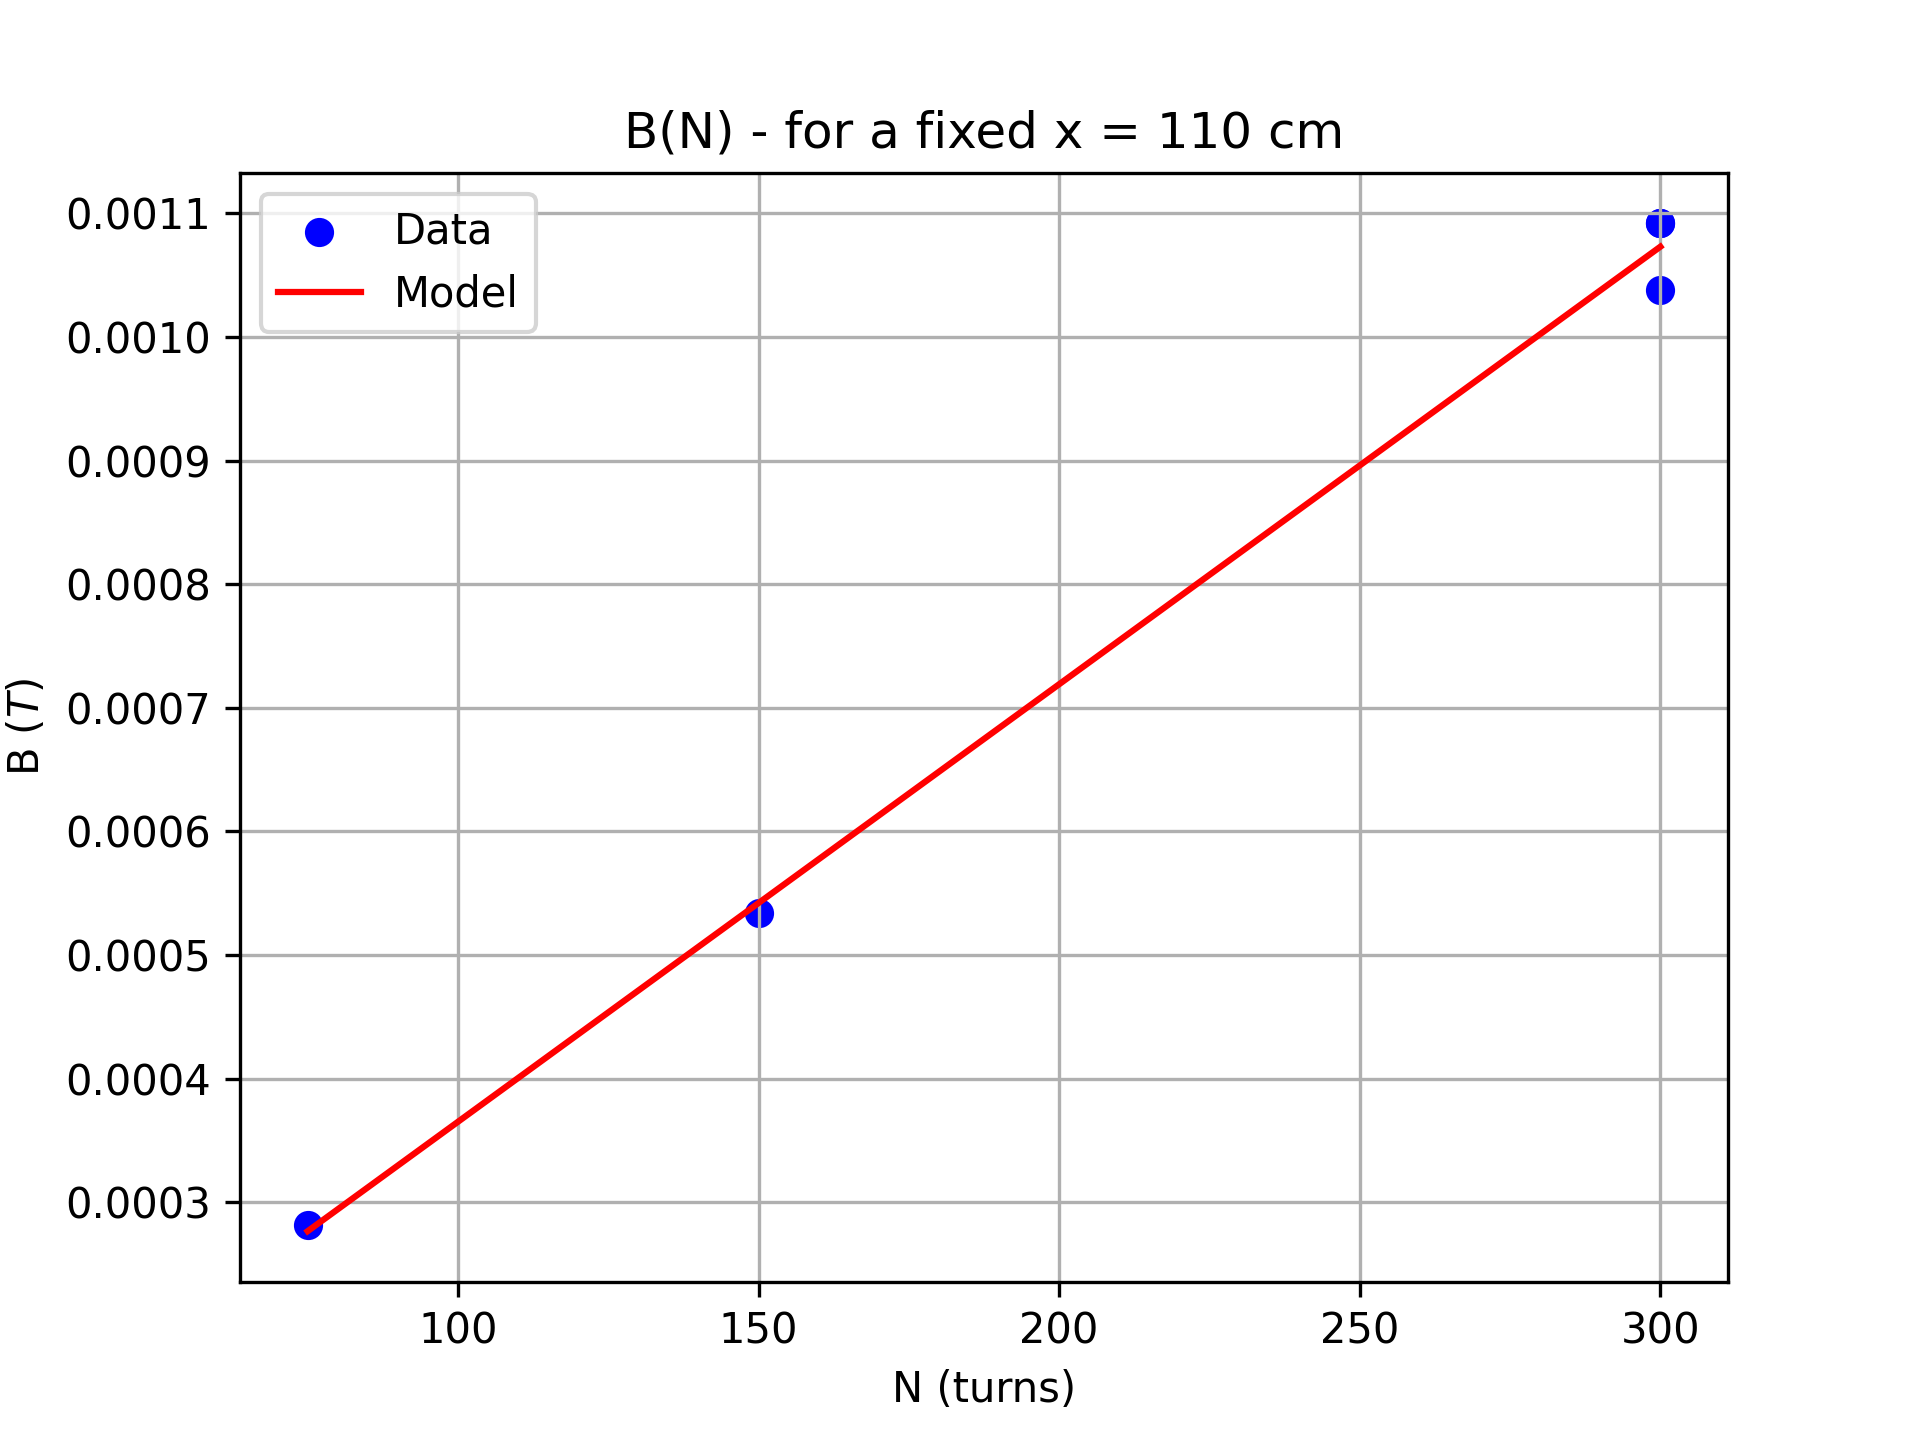
\includegraphics[width=\linewidth]{output_plots/B_vs_n_110cm.png}
    \caption{Relationship between magnetic field (\( B \)) and number of turns (\( N \)) for a fixed distance (\( x = 110 \, \text{mm} \)). The slope of the regression line is used to calculate \( \mu_0 \).}
    \label{fig:b_vs_turns}
    \end{figure}
    
    \begin{table}[H]
    \centering
    \caption{Computed Permeability for Solenoid Configurations}
    \label{tab:computed_mu}
    \begin{tabular}{ccc}
    \toprule
    Turns (\( N \)) & Magnetic Field (\( B \), \( mT \)) & Permeability (\( \mu \), \( \text{H/m} \)) \\
    \midrule
    75   & 0.282 & \( 1.203 \times 10^{-6} \) \\
    150  & 0.534 & \( 1.140 \times 10^{-6} \) \\
    300  & 1.092 & \( 1.165 \times 10^{-6} \) \\
    300 (\( 2a = 33 \, \text{mm} \)) & 1.092 & \( 1.165 \times 10^{-6} \) \\
    300 (\( 2a = 41 \, \text{mm} \)) & 1.038 & \( 1.107 \times 10^{-6} \) \\
    \bottomrule
    \end{tabular}
    \end{table}
    
    The table further demonstrates that the permeability values across various configurations consistently hover around the theoretical value. Slight deviations can be attributed to experimental uncertainties such as heating effects, non-idealities in the solenoid geometry, and environmental interference.
    
    Overall, these results validate our methodology for determining \( \mu_0 \) and affirm the robustness of the theoretical framework governing solenoids and their magnetic fields.
    
    

    \section{Discussion}
    The experimental results demonstrated a strong linear dependence of the magnetic field \( B \) inside the solenoid on the current \( I \) and the number of turns \( N \), consistent with the theoretical prediction given by \( B = \mu_0 n I \). The permeability of free space (\( \mu_0 \)) was determined using two approaches:
    
    \begin{enumerate}
        \item \textbf{Point-by-Point Calculation:} For each solenoid configuration, \( \mu_0 \) was calculated using the equation:
        \[
        \mu_0 = \frac{B \cdot l}{N \cdot I}.
        \]
        The results for different configurations showed excellent agreement, with the estimated values of \( \mu_0 \) consistently close to the theoretical value of \( 4\pi \times 10^{-7} \, \mathrm{H/m} \).
    
        \item \textbf{Slope-Based Method:} By analyzing the slope of the linear regression in the \( B \) vs. \( N \) graph at a fixed distance \( x = 110 \, \text{mm} \), the permeability was calculated using:
        \[
        \mu_0 = \frac{\text{slope} \cdot l}{I}.
        \]
        This method yielded an average \( \mu_0 \approx 1.13 \times 10^{-6} \, \mathrm{H/m} \), aligning closely with the theoretical value.
    \end{enumerate}
    
    Both methods highlight the reliability of the experimental setup and the consistency of the data. Minor deviations from the theoretical value can be attributed to:
    \begin{itemize}
        \item \textit{Heating Effects:} Higher currents may have caused slight changes in resistance and field strength.
        \item \textit{Measurement Uncertainties:} Precision limits of the Tesla meter and alignment errors in the setup.
        \item \textit{Environmental Factors:} Residual magnetic fields from external sources, including the Earth's field, may have influenced measurements.
    \end{itemize}
    
    Despite these challenges, the experiment robustly validated the theoretical framework governing solenoids and their magnetic fields.
    
    \section{Conclusion}
    This experiment successfully explored the relationship between current, coil geometry, and the magnetic field strength in a solenoid. The permeability of free space (\( \mu_0 \)) was determined using both point-by-point calculations and a slope-based regression model, with results aligning closely with the theoretical value of \( 4\pi \times 10^{-7} \, \mathrm{H/m} \). 
    
    Key findings include:
    \begin{itemize}
        \item The magnetic field inside the solenoid is linearly proportional to both the current \( I \) and the number of turns \( N \), as predicted by theory.
        \item The slope-based approach provided an efficient and accurate method for calculating \( \mu_0 \), further corroborating the experimental data.
    \end{itemize}
    
    Overall, the experiment demonstrated the strength of theoretical predictions in electromagnetism and the reliability of the experimental methodology. These results reinforce the importance of solenoids in practical applications, from inductors to transformers, and their foundational role in electromagnetic theory.
    
    \begin{thebibliography}{9}
        \bibitem{lab_manual}
            ISTANBUL UNIVERSITY, 
            \textit{Physics Laboratory II Experiment Book: Electricity and Magnetism}, 
            Department of Physics, 2024.
        
        \bibitem{github}
            \textit{Source code and additional experiments are available in the GitHub repository.} \\ 
            Access it at: \url{https://github.com/ibeuler/LAB-Reports}.
        
        \end{thebibliography}
        
        \begin{figure}[H]
            \centering
            \begin{minipage}{0.15\textwidth}
                \centering
                \qrcode[height=2cm]{https://github.com/ibeuler/LAB-Reports}
            \end{minipage}%
            \begin{minipage}{0.2\textwidth}
                \raggedright
                \caption{Access the GitHub repository for the lab manual, source code, and related experiments: \href{https://github.com/ibeuler/LAB-Reports}{\url{https://github.com/ibeuler/LAB-Reports}}.}
                \label{fig:qr}
            \end{minipage}
        \end{figure}
        

\end{document}